\documentclass{hbrs-ecta-report}

\usepackage{float}
\usepackage{placeins}
\usepackage{ngerman}
\usepackage[utf8]{inputenc}
\begin{document}

\conferenceinfo{H-BRS}{2017}

\title{Neuroevolution: Simple Genetic Algorithm}
\subtitle{}

\numberofauthors{2}
\author{
\alignauthor
Tim L"ugger, Jan Urfei
}

\date{today}
\maketitle
\begin{abstract}
Aufgabe: Implementiere einen Genetische Algorithmus und führe diesen 100 mal mit einer vorgegebenen Kostenfunktion aus. Ziel ist es das Minimum der egg Funktion zu finden.S	
\end{abstract}

\section{Der Genetische Algorithmus}
Der Genetische Algorithmus besitzt eine Population, welches eine Menge fester Größe an verschiedenen Lösungen ist. Diese Population wird pro Durchlauf verändert. Einen Durchlauf nennt man eine Generation. 
\\ 
\\
Als erstes wählt man ''zufällig'' Elternpaare für die nächste Generation aus. Für diese Auswahl gibt es verschiedene Verfahren auf die wir hier nicht näher eingehen. Diese Elternpaare werden verglichen und der Teil der den besseren Fitnesswert hat kommt in die neue Population der nächsten Generation. Der Beste (die Elite) der alten Generation wird einfach übernommen.
\\ 
\\
Danach werden aus der neu gebildeten Menge zu einer gewissen Wahrscheinlichkeit  2 Lösungen genommen, die zueinander vereint werden und eine neue Lösung bilden. Diesen Vorgang nennt man Crossover.
\\
\\
Nachdem Crossover nimmt man sich noch einen gewissen Prozentsatz aller Lösungen und mutiert diese, d.h. diese werden minimal zufällig verändert, sodass eine neue ähnliche Lösung entsteht.
\\
\\ 
Jetzt  hat sich eine neue Population gebildet, die die alte beste Lösung beinhaltet und neue ähnliche Lösungen, um vielleicht noch bessere zu finden. Die Populationsgröße, der Wahrscheinlichkeit zum mutieren und für den Crossover, sowie die Anzahl an Generationen sind Parameter, die das Ergebnis sehr stark beeinflussen können.
\section{Herangehensweise}
Die Anfangspopulation wird zufällig aus Koordinatenpaaren gebildet, die Innerhalb des gültigen Wertebereichs [-512 ; 512] liegen. Von allen Lösungen berechnen wir danach die Fitness. Als Kostenfunktion nutzen wir die Egg Funktion (Figure \ref{fig:egg}). 

\begin{figure}[h!]
	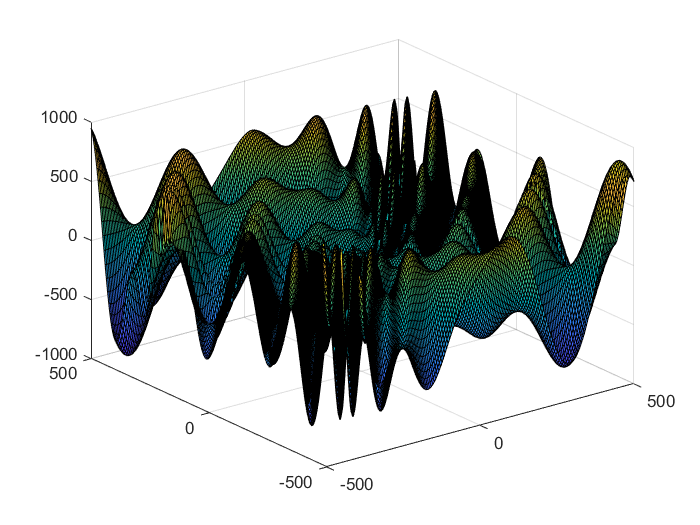
\includegraphics[width=\linewidth]{img/egg}
	\caption{3D Eggholder function: defined between -512 and 512}
	\label{fig:egg}
\end{figure}
Danach schnappen wir uns zwei zufällige Lösungen und stecken die bessere in die neue Population. Es werden alle Lösungen aus der alten Generation bis auf den Besten auf diese Art und Weise ersetzt.


\section{Unsere Ergebnisse}


\end{document}
}